% !TeX TXS-program:compile = txs:///pdflatex/[--shell-escape]

\documentclass[11pt, letterpaper]{article}

\usepackage{minted}
\usepackage[utf8]{inputenc}
\usepackage[T1]{fontenc}
\usepackage{lmodern}
\usepackage{graphicx}
\usepackage{longtable}
\usepackage{wrapfig}
\usepackage{rotating}
\usepackage{amsmath}
\usepackage{textcomp}
\usepackage{amssymb}
\usepackage{hyperref}
\usepackage[round]{natbib}
\usepackage{subcaption}


\title{\bfseries Tarea}
\author{Ángel García Báez}
\date{\today}
\setcounter{tocdepth}{3} 

\begin{document}
	
	% Página de presentación
	\begin{titlepage}
		\centering
		
\includegraphics[width=0.2\textwidth]{logo.png}\par
		\vspace{1cm}
		{\LARGE \bfseries Universidad Veracruzana \par}
		\vspace{1cm}
		{\Large Maestría en Inteligencia Artificial\par}
		\vspace{3cm}
		{\LARGE \bfseries Visión por Computadora \par}
		\vspace{1cm}
		{\Large \bfseries Tarea 6. Aplicación de LDA a la base de datos de pingüinos palmer en MATLAB para el caso de dos clases y para el caso multiclase. \par}
		\vfill
		{\Large \textit{Ángel García Báez}\par}
		\vspace{1cm}
		{\Large Profesor: Dr. Héctor Acosta Mesa y Dra. Adriana Laura López Lobato\par}
		\vfill
		{\Large \today \par}
	\end{titlepage}
	
	% Página exclusiva para la tabla de contenidos
	\newpage
	\tableofcontents
	\newpage
	
% Sección para el problema 1
\section{Objetivo de la práctica}
	
Se tiene la base de datos de pingüinos palmer, la cual representa las mediciones de 3 especies de pingüinos en distintas islas, a lo largo de distintos años, la cual tiene la siguiente estructura:


\begin{figure}[h!]
	\centering
	\begin{minipage}{1\textwidth}
		\centering
		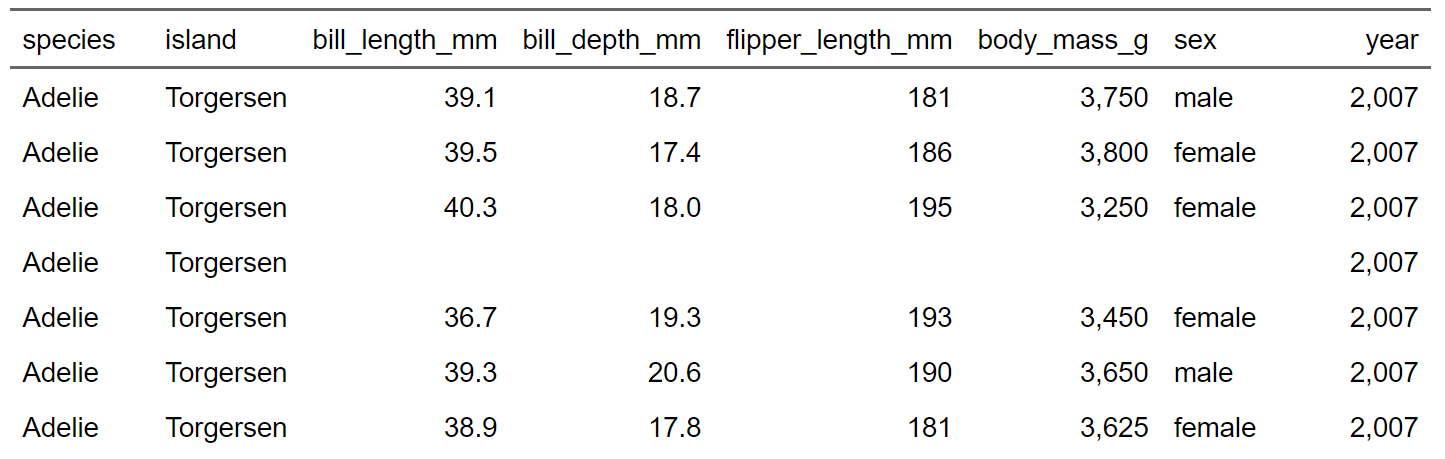
\includegraphics[width=\textwidth]{IMG/T1.png}
		\caption{Base de datos de los pingüinos palmer (primeros 5 casos)}
		\label{fig:f1}
	\end{minipage}\hfill
\end{figure}

La base esta compuesta por 344 observaciones y 8 variables (4 variables categóricas o de etiqueta y 4 variables numéricas continuas). Para efectos del desarrollo del documento, se tomaran en cuenta unicamente las 4 variables numéricas continuas (bill\_length, bill\_depth, flipper\_length y body\_mass) junto con la variable categórica de species para hacer el coloreado en los gráficos.

\newpage

La problemática que se desea abordar y  por la cual se quiere aplicar LDA es la siguiente: Se desea poder proyectar la información de las 4 dimensiones en un espacio de menor dimensionalidad, esto con la finalidad de poder observar gráficamente como se están comportando los datos.

Dada la naturaleza del LDA que es capaz de representar los datos en $k-1$ dimensiones, donde $k$ es la cantidad de grupos (en este caso, especies de pingüinos), se plantea el proyectar las aproximaciones en 1D y en 2D para el caso donde se tienen unicamente 2 especies y para el caso donde se tienen 3 especies respectivamente.

Con el objetivo de evidenciar lo difícil que es ver como se están comportando los datos a continuación se muestran los gráficos de dispersión tomando subconjuntos de las variables:

\begin{figure}[h!]
	\centering
	\begin{minipage}{1.1\textwidth}
		\centering
		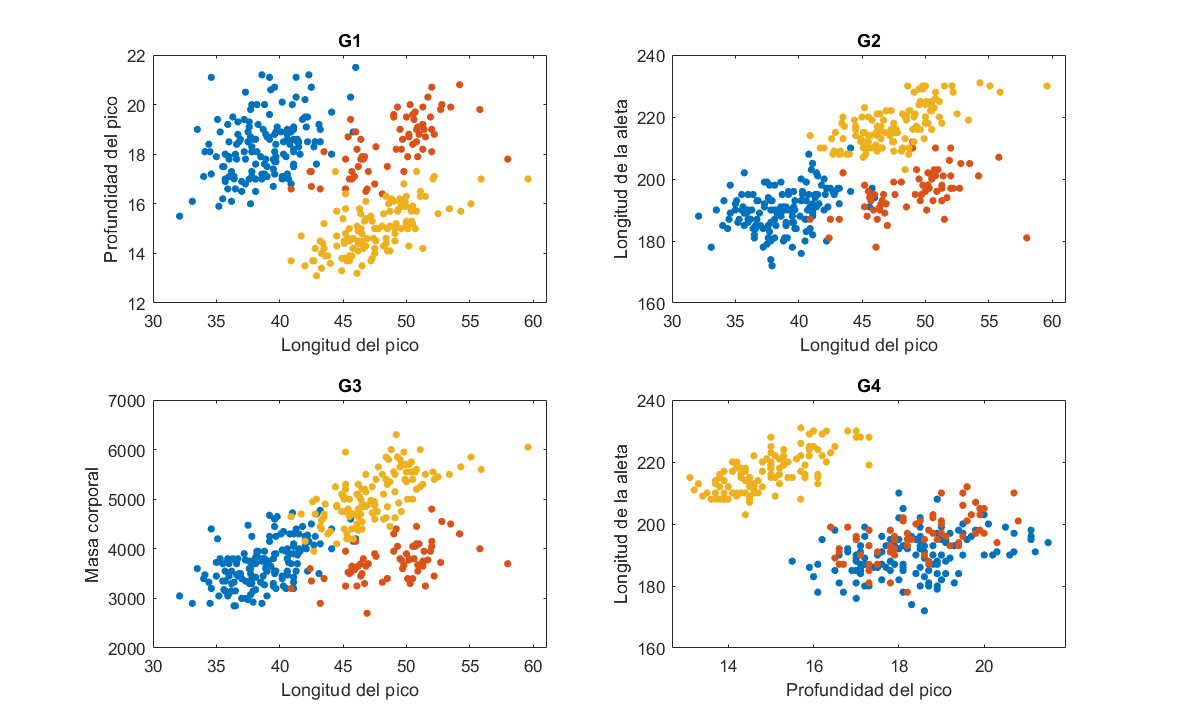
\includegraphics[width=\textwidth]{IMG/G1.png}
		\caption{Gráficos de dispersión bivariados.}
		\label{fig:f2}
	\end{minipage}\hfill
\end{figure}

Se puede observar que para algunos pares de variables, se alcanza a ver una separación clara de los datos por especies, sin embargo, al verlo desde otro par de variables, la cosa se vuelve difusa de distinguir, como es el caso del gráfico G4, en donde se esta mostrando el comportamiento de las variables de la profundidad del pico y el largo de la aleta.

\newpage

Por otro lado, se hizo la propuesta de modelarlos en 3 dimensiones, para observar como se comportan los datos en el espacio:

\begin{figure}[h!]
	\centering
	\begin{minipage}{1.1\textwidth}
		\centering
		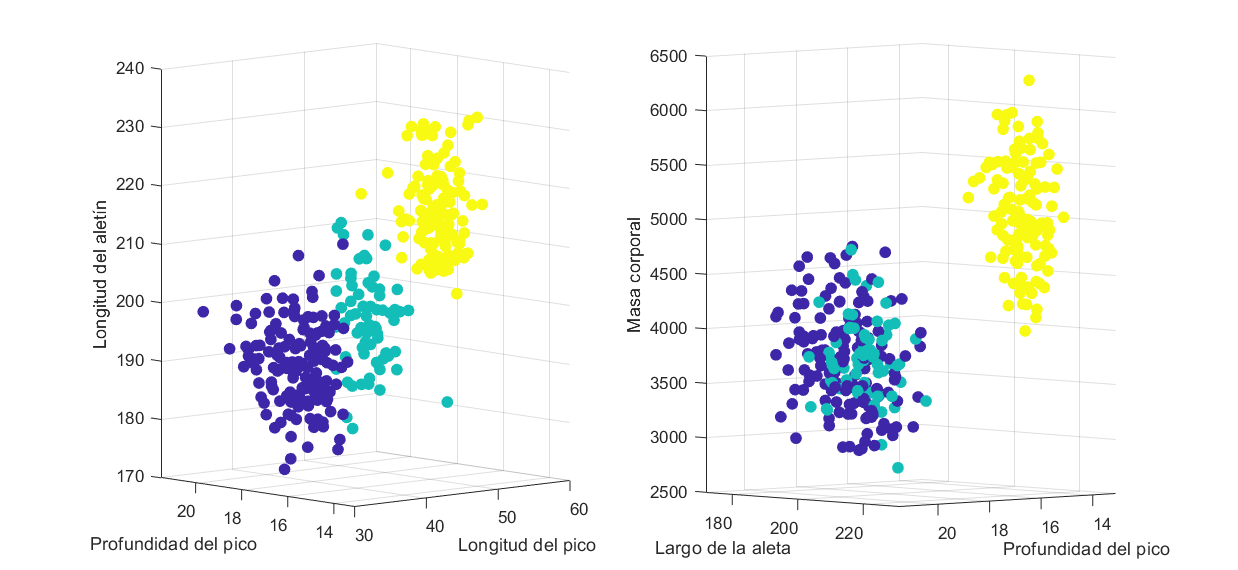
\includegraphics[width=\textwidth]{IMG/G2.png}
		\caption{Gráficos de dispersión multivariados.}
		\label{fig:f3}
	\end{minipage}\hfill
\end{figure}


En el primer gráfico se logra apreciar una separación distinguible entre los grupos de pingüinos dada su visualización mediante las variables de profundidad del pico, longitud del pico y longitud de la aleta. Por otro lado, en el gráfico de la derecha, se observa como un grupo esta perfectamente diferenciado del resto pero los 2 grupos restantes se encuentran sobre puestos uno con el otro, lo que los hace difíciles de separar usando las variables de profundidad del pico, largo de la aleta y masa corporal.

Es por ello que se quiere usar LDA para proyectar la información y reducir la dimensionalidad de los datos para observar mejor su comportamiento en 1 y 2 dimensiones.

	
	\newpage
	
	\section{Metodología}
	
El discriminante lineal es una técnica multivariada de aprendizaje supervisado que permite reducir la dimensionalidad de datos cuantitativos continuos que se encuentren etiquetados por una variable de clase, donde el resultado son $k-1$ combinaciones lineales donde proyectar los datos \cite{johnson2007}.

 Cabe mencionar que esto se hace bajo supuestos fuertemente ligados a que los conjuntos de datos por grupo siguen una distribución normal multivariada, tienen una matriz de varianzas y covarianzas similar distinta de la matriz nula y que son independientes entre sí.
	
Para ejecutar la técnica, es necesario tener identificados a la matriz de características $X$ y al vector de etiquetas o clases $Y$: 
	
	$$
	 \begin{matrix}
	 	X = \{x_1,x_2,\dots,x_n\} \\
	 	Y = \{y_1, y_2,\dots ,y_k\}
	 \end{matrix}
	$$
	
	Donde: 
	\begin{itemize}
		\item $X$ Es la matriz de datos de tamaño $N\times P$.
		\item $Y$ Es el vector que contiene las clases de tamaño $N\times 1 $.
	\end{itemize}
	

Una vez identificados los elementos fundamentales para dar inicio a la técnica, se procede a calcular la matriz de dispersión entre clases como sigue:

$$S_w = \sum_{i = 1}^{k} {(X_i-\mu_i)(X_i-\mu_i)' }$$

	Donde: 
	\begin{itemize}
		\item $S_w$ Es la matriz de dispersión entre clases de tamaño $P\times P$.
		\item $X_i$ Es la matriz de de características $X$ de la clase $i$-ésima de tamaño $N_i \times P$.
		\item $\mu_i$ Es el vector de medias de la matrix $X_i$ de tamaño $1\times P$.
		\item $k$ Es la cantidad de clases en el conjunto de datos.
	\end{itemize}

\newpage

Posteriormente, se procede a calcular la dispersión total presente en los datos como sigue:

$$S_t = {(X-\mu)(X-\mu)' }$$

Donde: 
\begin{itemize}
	\item $S_t$ Es la matriz de dispersión de todo el conjunto de datos sin considerar clases de tamaño $P\times P$.
	\item $X$ Es la matriz de de características $X$ de tamaño $N \times P$.
	\item $\mu$ Es el vector de medias de la matrix $X$ de tamaño $1\times P$.
\end{itemize}

Una vez hecho el calculo de la matriz de dispersión global $S_t$, se obtiene por diferencia la matriz de dispersión dentro de clases como sigue:

$$S_b = S_t-S_w$$

Donde: 

\begin{itemize}
	\item $S_b$ Es la matriz de dispersión entre clases de tamaño $P\times P$.
	\item $S_t$ Es la matriz de de dispersión de los datos de tamaño $P \times P$.
	\item $S_w$ Es la matriz de de dispersión dentro de clases de tamaño $P \times P$.
\end{itemize}

Una vez determinadas las matrices de dispersión entre clases y dentro de clases, el siguiente paso es maximizar el criterio de Fisher, el cual busca que las clases esten lo más separadas posibles y que la varianza dentro de las clases sea la más pequeña posible como se muestra a continuación:

$$MAX \quad J(W)  = \frac{|W^TS_bW|}{|W^TS_wW|}$$

Donde: 

\begin{itemize}
	\item $J(W)$ Es el criterio de Fisher.
	\item $W$ Es la matriz de vectores propios de tamaño $P \times P$.
	\item $S_b$ Es la matriz de dispersión entre clases de tamaño $P\times P$.
	\item $S_w$ Es la matriz de de dispersión dentro de clases de tamaño $P \times P$
\end{itemize}

\newpage

Para encontrar los valores de la matriz $W$ que logran maximizar el criterio de fisher, se resuelve como un problema de valores propios generalizados como se muestra:

$$S_bW = \lambda S_wW$$

Donde: 

\begin{itemize}
	\item $W$ Es la matriz de vectores propios de tamaño $P \times P$.
	\item $S_b$ Es la matriz de dispersión entre clases de tamaño $P\times P$.
	\item $S_w$ Es la matriz de de dispersión dentro de clases de tamaño $P \times P$
	\item $\lambda$ Es el vector de valores propios de tamaño $1 \times P$.
\end{itemize}

El resultado esperado son $P$ valores propios que indican cuanta varianza acumula cada una de las componentes en el nuevo sistema de coordenadas donde se van a proyectar los datos originales y $P$ vectores propios que serán los ejes sobre los cuales se proyecten los datos.

Para hacer la proyección de los datos centrados en el nuevo sistema, basta con aplicar la siguiente operación matricial con los vectores propios encontrados:

$$Z = XW$$

Donde: 
\begin{itemize}
	\item $Z$ Son las proyecciones de las características X sobre los vectores W.
	\item $X$ Es la matriz de características de tamaño $N \times P$.
	\item $W$ es la matriz de vectores propios de tamaño $P \times P$ .
\end{itemize}

Finalmente, se calcula la variabilidad explicada por cada componente mediante los valores propios como sigue:

$$VE = 100*\frac{\lambda_i}{\sum_{i = 1}^P{\lambda_i}}$$

Donde: 

\begin{itemize}
	\item $VE$ Es la variabilidad explicada por el $i$-ésimo valor propio.
	\item $\lambda_i$ Es el $i$-ésimo valor propio.
\end{itemize}

Cabe mencionar que los valores propios conservan la siguiente propiedad:

$$\lambda_1 \geq \lambda_2 \geq \dots \geq \lambda_P$$

Nota importante: Debido a que el discriminante lineal toma en cuenta la cantidad de clases con las que se esta trabajando, logra reducir aun más el número de dimensiones tal que solo se van a proyectar $k-1$ dimensiones como resultado.
Pese a que operativamente se generen $P$ valores y vectores propios, la realidad es que solo $k-1$ valores propios van a ser distintos de 0, esto implica que los  vectores propios asociados a esos $k-1$ valores propios distintos de 0 van a ser los proyectados y que concentran la información original en una menor dimensionalidad.

Como ejemplo, si se tienen 2 clases y 4 variables, el sistema va a calcular 4 valores propios y 4 vectores propios, pero solo $2-1$ valores propios van a ser distintos de 0, por lo que toda la variabilidad explicada recae en un solo vector propio, por lo que la salida de los datos sera su proyección en 1 dimensión.

Otro ejemplo, si se tienen 3 clases y 4 variables, el sistema va a calcular 4 valores propios y 4 vectores propios, pero solo $3-1$ valores propios van a ser distintos de 0, por lo que toda la variabilidad explicada recae en dos vectores propios, por lo que la salida de los datos sera su proyección en 2 dimensiones.

\newpage

A continuación, se aplico un breve pre-procesamiento de los datos:


\begin{itemize}
	\item Se identificaron y eliminaron las filas con valores faltantes (2 filas eliminadas)
	\item Se guardo en $X$  las variables numéricas de longitud del pico, profundidad del pico, largo de la aleta y masa corporal.
	\item Se guardo en $Y$ las etiquetas de la especie a la que pertenecen los individuos.
\end{itemize}

Posteriormente, se aplico LDA para reducir dimensionalidad en 2 casos: 


\begin{itemize}
	\item Para los datos recortados unicamente con 2 especies de pingüinos (Adelie y Chinstrap)
	\item Para el caso de la base de datos completa que contempla las 3 especies de pingüinos (Adelie, Chinstrap y Gentoo).
\end{itemize}


\newpage
	
\section{Resultados para dos clases}

A continuación se muestran los resultados obtenidos para los datos de los pingüinos palmer en matlab cuando se trabajan con 2 clases. 

\subsection{Vectores de medias}

Se muestra el vector de medias obtenido para las variables de Longitud del pico, profundidad del pico, longitud de la aleta y la masa corporal para la especie Adelie, Chinstrap y el vector de medias general:

$$
\begin{matrix}
	\mu_{Adelie} =  &\{38.7914 & 18.3464 & 189.9536 & 3700.662\}	 \\
	\mu_{Chinstrap} = & \{48.8338 & 18.4206 & 195.8235 & 3733.088\}	 \\
	\mu = & \{41.90959 & 18.36941 & 191.77626 & 3710.73059 \}	 
\end{matrix}
$$


Se observa la evidente diferencia de las escalas entre las variables, siendo la masa corporal la que tiene valores más altos respecto al resto de variables en su media para los 3 vectores.

\subsection{Matriz de dispersión dentro de clases}

Aplicando la definición para la matriz de dispersión dentro de las clases descrita previamente, se obtuvo la siguiente matriz:

$$
S_w = 
\begin{bmatrix}
1811.1510 & 356.3029 & 1603.6456 & 144719.76\\
356.3029 & 308.4067 & 681.8716 & 65889.04\\
1603.6456 & 681.8716 & 9822.5578 & 328426.69\\
144719.7580 & 65889.0407 & 328426.6946 & 41439235.25
\end{bmatrix}
$$

Se observa como las varianzas y covarianzas de la matriz son mayores en los pares donde esta involucrada la variable de masa corporal (variable 4), mientras que por otro lado, resultan menores en aquellas parejas donde se encuentra involucrada la variable ancho del pico (variable 2).

\newpage

\subsection{Matriz de dispersión entre clases}

Aplicando la definición para la matriz de dispersión entre las clases descrita previamente, se obtuvieron las siguientes matrices (la matriz de dispersión global y la matriz de dispersión entre clases):

$$
S_t = 
\begin{bmatrix}
	6539.6099 & 391.2542 & 4367.4699 & 159987.5 \\
	391.2542 & 308.6650 & 702.3009 & 66001.9 \\
	4367.4699 & 702.3009 & 11438.0365 & 337350.8 \\
	159987.4658 & 66001.8950 & 337350.7991 & 41488533.1
\end{bmatrix}
$$

$$
S_b = S_t-S_w = 
\begin{bmatrix}
4728.4588 & 34.9513 & 2763.8242 & 15267.7078 \\
34.9513 & 0.2583 & 20.4294 & 112.8543 \\
2763.8242 & 20.4294 & 1615.4787 & 8924.1045 \\
15267.7078 & 112.8543 & 8924.1045 & 49297.8596
\end{bmatrix}
$$

\newpage


\subsection{Valores y vectores propios}

Se construye la matriz que representa el criterio de Fisher a Maximizar:

$$S = S_w^{-1}S_b = 
\begin{bmatrix}
3.7501 & 0.0277 & 2.1919 & 12.1085 \\
-2.4144 & -0.0178 & -1.4112 & -7.7957 \\
0.1823 & 0.0013 & 0.1065 & 0.5885 \\
-0.0103 & -0.0001 & -0.0060 & -0.0334
\end{bmatrix}
$$

Posteriormente, se calculan los valores y vectores propios como resultado de la resolución de la matriz S como un problema de valores y vectores propios generalizado como sigue:

$$\lambda = 
\begin{bmatrix}
	3.8054 &
	0 &
	0 &
	0 
\end{bmatrix}
$$

$$ W = 
\begin{bmatrix}
0.8401 & 0.2773 & -0.0506 & -0.0018 \\
-0.5409 & 0.8034 & -0.9958 & -1.0000 \\
0.0408 & -0.5268 & 0.0766 & 0.0085 \\
-0.0023 & 0.0076 & 0.0041 & 0.0013
\end{bmatrix}
$$

Se observa como el primer vector propio de la un mayor peso a la variable de la longitud del pico para hacer la proyección en el nuevo espacio, siendo la masa corporal la que menor peso tiene en este nuevo eje.

Haciendo las cuentas, a continuación se muestra cuanta variabilidad explica cada componente:

$$VE = 
\begin{bmatrix}
	100 &
	0 &
	0 &
	0 
\end{bmatrix}
$$

Recordando que solo vamos a tener 1 vector característico que proyecta a los datos y 1 solo valor característico distinto de 0 asociado a dicho vector, lo anterior se puede re-escribir dicho vector propio y vector propio como sigue:

$$ W = 
\begin{bmatrix}
	0.8401 & -0.5409 & 0.0408 & -0.0023 
\end{bmatrix}, \quad \lambda = 3.8054, \quad VE = 100\%
$$

El vector $W$ proyecta en un solo nuevo eje a la matriz de características $X$, dicho vector proyector explica un 100\% de la variabilidad de los datos.

 

\newpage

\subsection{Proyección de las nuevas componentes}

A continuación se muestra una pequeña fracción de los datos al ser proyectados sobre el nuevo sistema creado con ayuda de los vectores propios:

\begin{figure}[h!]
	\centering
	\begin{minipage}{0.8\textwidth}
		\centering
		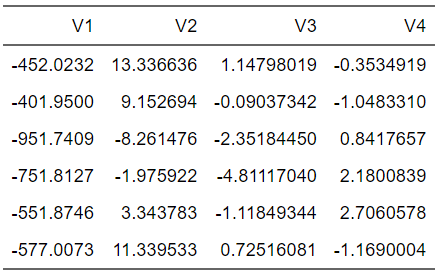
\includegraphics[width=0.3\textwidth]{IMG/T2.png}
		\caption{Matriz de caracteristicas $X$ proyectadas sobre 1 nuevo eje).}
		\label{fig:f4}
	\end{minipage}\hfill
\end{figure}

El nuevo sistema de proyección consta unicamente de un eje en donde se proyectaron los datos, debido a que solo el primer eje resulto explicar el 100\% de la variabilidad de los datos.

\newpage

\subsection{Proyección en 1D}

Debido a que el primer y único eje de la proyección de los datos es el único que se tiene para cuando hay 2 clases, se procede a proyectarlo en un espacio unidimensional para observar como se comporta:

\begin{figure}[h!]
	\centering
	\begin{minipage}{1.1\textwidth}
		\centering
		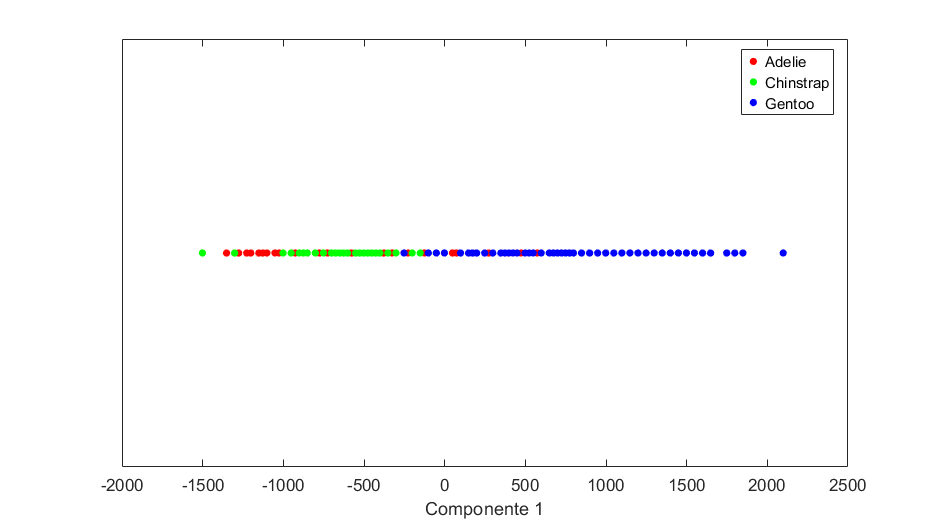
\includegraphics[width=\textwidth]{IMG/G3.png}
		\caption{Proyección en 1D sobre el eje 1.}
		\label{fig:f5}
	\end{minipage}\hfill
\end{figure}

El gráfico de la proyección unidimensional del discriminante lineal muestra un traslape entre las especies, siendo que Algunos Adelie tienen caracteristiacs que los hacen parecer Chinstrap y biceversa. 

\newpage

\section{Resultados para tres clases}

A continuación se muestran los resultados obtenidos para los datos de los pingüinos palmer en matlab cuando se trabajan con las 3 clases del conjunto de datos. 

\subsection{Vectores de medias}

Se muestra el vector de medias obtenido para las variables de Longitud del pico, profundidad del pico, longitud de la aleta y la masa corporal para la especie Adelie, Chinstrap, Gentoo y el vector de medias general:

$$
\begin{matrix}
	\mu_{Adelie} =  &\{38.7914 & 18.3464 & 189.9536 & 3700.662\}	 \\
	\mu_{Chinstrap} = & \{48.8338 & 18.4206 & 195.8235 & 3733.088\}	 \\
	\mu_{Gentoo} = & \{47.5049 & 14.9821 &  217.1870  & 5076.016\}	 \\
	\mu = & \{43.92193 & 17.15117 & 200.91520 & 4201.75439\}	 
\end{matrix}
$$
 



Se observa la evidente diferencia de las escalas entre las variables, siendo la masa corporal la que tiene valores más altos respecto al resto de variables.

\subsection{Matriz de dispersión dentro de clases}

Aplicando la definición para la matriz de dispersión dentro de las clases descrita previamente, se obtuvo la siguiente matriz:

$$
S_w = 
\begin{bmatrix}
2969.8881 & 593.6636 & 3215.733 & 271554.1 \\
593.6636 & 425.8673 & 1230.383 & 109283.8 \\
3215.7334 & 1230.3829 & 14953.257 & 608678.3 \\
271554.1482 & 109283.7765 & 608678.321 & 72443483.2
\end{bmatrix}
$$

Se observa como las varianzas y covarianzas de la matriz son mayores en los pares donde esta involucrada la variable de masa corporal (variable 4), mientras que por otro lado, resultan menores en aquellas parejas donde se encuentra involucrada la variable ancho del pico (variable 2).


\newpage

\subsection{Matriz de dispersión entre clases}

Aplicando la definición para la matriz de dispersión entre las clases descrita previamente, se obtuvieron las siguientes matrices (la matriz de dispersión global y la matriz de dispersión entre clases):

$$
S_t = 
\begin{bmatrix}
10164.2055 & -864.1738 & 17178.136 & 888506.8 \\
-864.1738 & 1329.8345 & -5528.616 & -254853.2 \\
17178.1360 & -5528.6161 & 67426.541 & 3350125.9 \\
888506.8421 & -254853.2018 & 3350125.877 & 219307697.4
\end{bmatrix}
$$

$$
S_b = S_t-S_w = 
\begin{bmatrix}
7194.317 & -1457.8374 & 13962.403 & 616952.7 \\
-1457.837 & 903.9672 & -6758.999 & -364137.0 \\
13962.403 & -6758.9990 & 52473.284 & 2741447.6 \\
616952.694 & -364136.9782 & 2741447.557 & 146864214.2
\end{bmatrix}
$$

\newpage


\subsection{Valores y vectores propios}

Se construye la matriz que representa el criterio de Fisher a Maximizar:

$$S = S_w^{-1}S_b = 
\begin{bmatrix}
3.2165 & -0.4000 & 4.6163 & 176.8832 \\
-12.5988 & 6.5009 & -49.9444 & -2631.6653 \\
0.9866 & -0.5443 & 4.1384 & 219.9163 \\
0.0072 & -0.0088 & 0.0611 & 3.4865
\end{bmatrix}
$$

Posteriormente, se calculan los valores y vectores propios como resultado de la resolución de la matriz S como un problema de valores y vectores propios generalizado como sigue:

$$\lambda = 
\begin{bmatrix}
	15.0192 &
	2.3231 &
	0 &
	0 
\end{bmatrix}
$$

$$ W = 
\begin{bmatrix}
-0.0846 & -0.9982 & -0.0375 & 0.2808 \\
0.9930 & -0.0502 & -0.9943 & -0.8166 \\
-0.0825 & 0.0322 & 0.0997 & -0.5043 \\
-0.0012 & 0.0041 & -0.0042 & 0.0062
\end{bmatrix}
$$

Se observa como el primer vector propio tiene un mayor peso en la variable de la longitud del pico mientras que en el segundo vector propio, el mayor peso lo recibe la variable de la longitud del pico. Siendo la longitud de la masa corporal la que menos peso tiene en cada uno de los respectivos vectores.

Haciendo las cuentas, a continuación se muestra cuanta variabilidad explica cada componente:

$$VE = 
\begin{bmatrix}
	86.6046  &
	13.3954  &
	0 &
	0 
\end{bmatrix}
$$

Recordando que solo los primeros 2 vectores característicos proyectan los datos en un nuevo espacio de 2 dimensiones, esto se refleja en la variabilidad explicada con los valores propios, donde el primer nuevo eje explica el 86.6\% la variabilidad de los datos y el segundo explica el 13.4\%. A raiz de esto, solo importan los primeros 2 valores propios y vectores propios, por lo que se re-escriben los resultados como sigue:

 
 



$$ W = 
\begin{bmatrix}
	-0.0846 & 0.9930 & -0.0825 & -0.0012  \\\
	-0.9982 & -0.0502 & 0.0322  & 0.0041
\end{bmatrix}, \quad \lambda =[15.0192, 2.3231] \quad VE = [86.6064, 13.3954]\%
$$



\newpage

\subsection{Proyección de las nuevas componentes}

A continuación se muestra una pequeña fracción de los datos al ser proyectados sobre el nuevo sistema creado con ayuda de los vectores propios significativos obtenidos:

\begin{figure}[h!]
	\centering
	\begin{minipage}{0.8\textwidth}
		\centering
		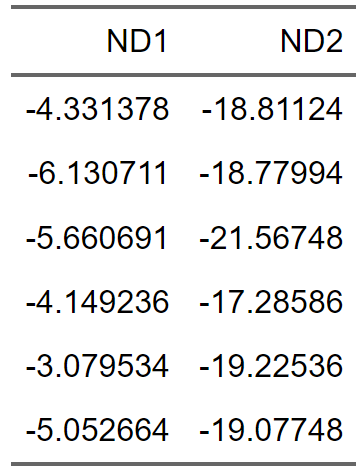
\includegraphics[width=0.6\textwidth]{IMG/T3.png}
		\caption{Base de datos centrada y proyectada sobre los vectores propios (primeros 6 casos).}
		\label{fig:f6}
	\end{minipage}\hfill
\end{figure}

Se observa como en los 2 nuevos ejes encontrados, los datos son proyectados hacia valores negativos.

\newpage

\subsection{Proyección en 2D}

Debido a que entre la primera y la segunda nueva dimensión se explica un 100\% de la variabilidad, a continuación se muestran sus proyecciones en un gráfico de dispersión: 

\begin{figure}[h!]
	\centering
	\begin{minipage}{1.1\textwidth}
		\centering
		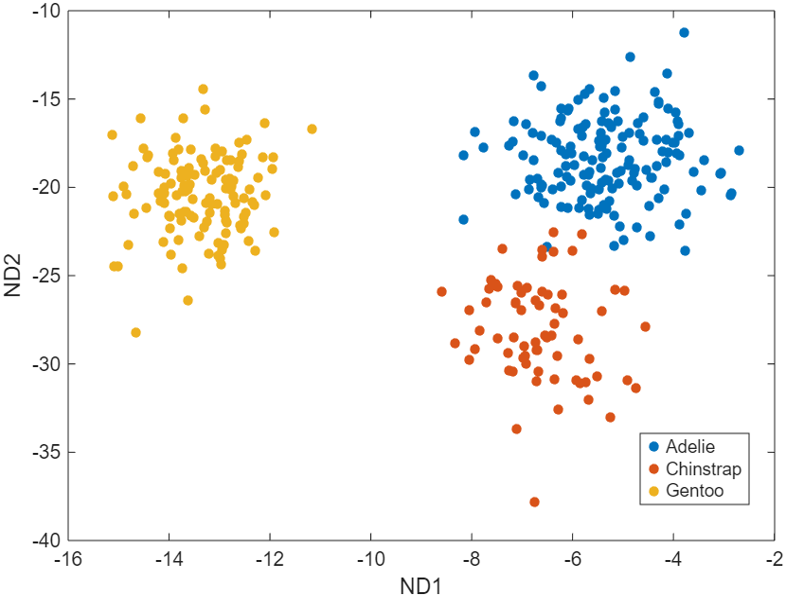
\includegraphics[width=\textwidth]{IMG/G6.png}
		\caption{Proyección en 2D sobre los nuevos ejes.}
		\label{fig:f7}
	\end{minipage}\hfill
\end{figure}

El gráfico muestra una proyección de los datos en donde se observa claramente la separación de la especie Gentoo respecto a las demás, mientras que la separación entre Adelie y Chinstrap es más evidente que en las gráficas mostradas al inicio del documento. El discriminante cumple bien su función de reducir la dimensionalidad y proyectar los datos originales en un nuevo espacio donde sea más evidente la separabilidad de los mismos.


\newpage
	
\section{Conclusiones}
	
Tras la exploración e implementación del algoritmo para la obtención del LDA, la tecnica reporta resultados bastante buenos al reducir la dimensionalidad de un conjunto de 4 dimensiones al lograr proyectarlo unicamente en 2, manteniendo entendible y explicable quienes son las variables de mayor peso en cada nueva dimensión para lograr dicha separabilidad.

Funciona bien a rasgos generales, puesto que como se observo en los resultados, la especie de Adelie y Chinstrap estan mezcladas entre sí, efecto que se logra atenuar mediante LDA al momento de visualizar los datos.

Por otro lado, aquí se trabajo el caso para 2 y 3 grupos, que son los que finalmente determinan cuantos ejes nuevos van a resultar del proceso, pero el problema se complica cuando se tienen 5 o más grupos, puesto que no es posible visibilizar los 4 tentativos nuevos ejes al mismo tiempo, por lo que seria necesario buscar o proponer alternativas que preserven la consistencia de los datos y puedan ser fácilmente representados en espacios de a lo más 3 dimensiones aunque se tengan 5 o más grupos.

Finalmente, la presencia de normalidad, homocedasticidad e independencia para los datos se asumió para este ejemplo, es importante la verificación de dichos supuestos debido a que la técnica clásica esta supuesta a ellos, en caso de no cumplirse, el proceso puede presentar problemas como matrices singulares no invertibles y de ultimas, que los resultados e inferencias obtenidos carezcan de 
robustez.
\newpage

	
\section{Referencias}  % Sección numerada de referencias
\bibliographystyle{apalike}  % Estilo de citas (puedes cambiarlo)
\bibliography{Biblio}        % Nombre del archivo BibTeX (sin extensión)

\newpage
	
\section{Anexos}	
\subsection{Implementación de la exploración y el LDA en MATLAB}
\begin{minted}[linenos,firstnumber=1]{matlab}
%% Cargar la base de datos en formato CSV %%
ruta = "penguins.csv";
datos = readtable(ruta); % Leer el archivo CSV en una tabla
size(datos); % Ver el tamaño de los datos
% 1 etiqueta de clasificación (Species)
% 3 características categóricas (Isla, sexo y año de observación)
% 4 variables continuas: bill length, bill depth, fliper y bodymass
% Filtrar solo las columnas numéricas y eliminar filas con datos faltantes
indices = find(any(isnan(datos{:, 4:7}), 2)); % Buscar filas con valores NaN en las columnas 4 a 7
datos1 = datos;
datos1(indices, :) = []; % Eliminar esas filas
% Extraer las variables numéricas y la especie para el gráfico
% Extraer las variables numéricas y la especie para el gráfico
especie = datos1.species; % Columna 'species' con las etiquetas de especies
% Convertir la columna 'especie' en un vector de tipo categorical
especie = categorical(especie); % Convertir a tipo categorical, que gscatter entiende
datos1 = table2array(datos1(:, 4:7)); % Convertir las columnas 4 a 7 a un arreglo numérico
%% Gráficos descriptivos %%
% Graficar el gráfico de dispersión usando gscatter
% Longitud del pico y ancho del pico
subplot(2,2,1)
gscatter(datos1(:,1), datos1(:,2), especie,"filled"); 
xlabel('Longitud del pico'); % Etiqueta del eje x
ylabel('Profundidad del pico'); % Etiqueta del eje y
title('G1'); % Título del gráfico
% Longitud del pico y longitud de la aleta %
subplot(2,2,2)
gscatter(datos1(:,1), datos1(:,3), especie,"filled");
xlabel('Longitud del pico'); % Etiqueta del eje x
ylabel('Longitud de la aleta'); % Etiqueta del eje y
title('G2'); % Título del gráfico
% Longitud del pico y masa corporal
subplot(2,2,3)
gscatter(datos1(:,1), datos1(:,4), especie,"filled");
xlabel('Longitud del pico'); % Etiqueta del eje x
ylabel('Masa corporal'); % Etiqueta del eje y
title('G3'); % Título del gráfico
% Ancho del pico y Longitud de la aleta
subplot(2,2,4)
gscatter(datos1(:,2), datos1(:,3), especie,"filled");
xlabel('Profundidad del pico'); % Etiqueta del eje x
ylabel('Longitud de la aleta'); % Etiqueta del eje y
title('G4'); % Título del gráfico
%% Exploración en 3D %&
% Crear un gráfico 3D
subplot(1,2,1)
scatter3(datos1(:,1), datos1(:,2), datos1(:,3), 50, especie, 'filled'); 
% Ajustar etiquetas y título
xlabel('Longitud del pico');
ylabel('Profundidad del pico');
zlabel('Longitud del aletín');
title('');
subplot(1,2,2)
scatter3(datos1(:,2), datos1(:,3), datos1(:,4), 50, especie, 'filled'); 
% Ajustar etiquetas y título
xlabel('Profundidad del pico');
ylabel('Largo de la aleta');
zlabel('Masa corporal');
title('');
% Mostrar la leyenda de colores
% Guardar como archivo PNG

%% FUNCIÓN LDA %%
function resu = LDA(X, Y)
	% Asegúrate de que X es una matriz
	X = double(X);    
	% Número de variables (columnas)
	nc = size(X, 2);
	% Clases únicas
	clas = unique(Y);
	nr = length(clas); % número de clases    
	% Inicializar matrices
	medias = zeros(nr, nc);
	Sw = zeros(nc, nc);
	for i = 1:nr
		% Subconjunto para la clase k-ésima
		mini1 = X(Y == clas(i), :);        
		% Vector de medias clase k
		medias(i, :) = mean(mini1, 1);        
		% Matriz de covarianza clase k
		centered = mini1 - medias(i, :);
		Sn = centered' * centered;        
		% Acumular la varianza dentro de clase
		Sw = Sw + Sn;
	end
	% Vector de medias global
	m = mean(X, 1);
	% Dispersión total
	centered_global = X - m;
	St = centered_global' * centered_global;
	% Matriz de dispersión entre clases
	Sb = St - Sw;
	% Matriz S = inv(Sw) * Sb
	S = inv(Sw) * Sb;
	% Eigenvalores y eigenvectores
	[V, D] = eig(S);
	[eigenvalues, idx] = sort(diag(D), 'descend');
	V = V(:, idx);
	% Varianza explicada
	VE = round(100 * eigenvalues / sum(eigenvalues), 4);
	% Filtrar vectores con varianza explicada significativa
	DS = VE > 0.0001;
	SV = V(:, DS);
	% Proyección de los datos
	Z = X * SV;
	% Renombrar las columnas
	for i = 1:size(Z, 2)
		colnames{i} = ['ND', num2str(i)];
	end
	% Armar resultado
	resu.varianza = VE;
	resu.coeficientes = SV;
	resu.proyecciones = array2table(Z, 'VariableNames', colnames);
end
%% Caso para 2 grupos (Adelie y Chinstrap)
X1 = datos1(Y ~= "Gentoo",:);
Y1 = especie(Y ~= "Gentoo");
%% Aplicar el LDA %%
salida1 = LDA(X1,Y1)
% Varianza explicada
salida1.varianza
% Vectores propios
salida1.coeficientes
% Proyecciones
Z1 = table2array(salida1.proyecciones);
%% Crear una dispersión en 1D (todos los puntos con la misma Y)
y = zeros(size(Z1, 1), 1); % Todos los puntos en Y=0
gscatter(Z1, y, Y1, 'rgb', '.', 15);
xlabel('ND1');
yticks([]); % Eliminar marcas del eje Y
ylabel('');
title('');
%% Caso para 3 grupos (Adelie, Chinstrap y Gentoo)
X2 = datos1;
Y2 = especie;
%% Aplicar el LDA %%
salida2 = LDA(X2,Y2)
% Varianza explicada
salida2.varianza
% Vectores propios
salida2.coeficientes
% Proyecciones
Z2 = table2array(salida2.proyecciones) 
%% Gráficar en 2D %%
gscatter(Z2(:,1), Z2(:,2), Y2,"filled");
xlabel('ND1'); % Etiqueta del eje x
ylabel('ND2'); % Etiqueta del eje y
title(''); % Título del gráfico
\end{minted}
	
	
	
	
\end{document}

